\documentclass[a4paper,10pt]{article}
\usepackage[utf8]{inputenc}
\usepackage[english]{babel}
\usepackage{apacite}
 
\usepackage[nottoc]{tocbibind}

%Imagenes
\usepackage{graphicx}
\graphicspath{{./images/}}

%Espacio de interlineado
\usepackage{setspace}
\doublespacing



\begin{document}


\begin{center}
\begin{Large}
Universidad Nacional Autónoma de México\\
Facultad de Ciencias\\
\end{Large}
\begin{LARGE}
Proyecto para la Opción de Titulación por Reporte de Trabajo Profesional\\
RobotSAI: Sistema para automatizar las órdenes de reposición en el portal SAI del IMSS\\*[1ex]
\end{LARGE}

Alumno: Ernesto Carrillo Espinosa - No. de cuenta: 300138647\\
Tutor: M. en I. Karla Ramírez Pulido\\*[1ex]
\today
\end{center}


\section{Introducción}
El Instituto Mexicano del Seguro Social (IMSS) cuenta con proveedores que se encargan de surtir los medicamentos a sus respectivas clínicas y hospitales; el documento digital en el cual se asienta la solicitud de un medicamento es llamada orden de reposición, este documento contiene la descripción del medicamento y el lugar en donde es solicitada la entrega del mismo. El IMSS hace llegar a los proveedores las órdenes de reposición a través del portal web llamado Sistema de Abasto Institucional (SAI), donde, el proveedor a su vez puede confirmar dentro del portal la recepción de las órdenes de reposición. El proveedor realiza dos flujos, \textbf{envío de órdenes de reposición} y \textbf{verificación de órdenes de reposición canceladas}:
\begin{itemize}
\item \textbf{Envío de órdenes de reposición}: un operador debe acceder al portal SAI, con un usuario y contraseña asignados por el IMSS, posteriormente debe dirigirse a la sección \textit{Contestación a Órdenes de Reposición} que es donde se muestra un listado con las órdenes de reposición emitidas por el IMSS que aún no han sido atendidas; el operador manualmente ingresa cada orden de reposición los datos requeridos como la cantidad de unidades que enviará, fechas de fabricación y caducidad, a esto se le conoce como responder la orden reposición. En el listado de órdenes de reposición de la sección \textit{Contestación a Órdenes de Reposición} se muestra la opción ``enviar'' cuando una orden de reposición ha sido \textit{contestada}, dicho lo anterior, el operador selecciona la opción ``enviar'' de cada una de las órdenes de reposición que ha contestado, el portal muestra un formato de acuse de recibo, el operador extraer datos de interés que se muestran en el acuse y hace una impresión de pantalla. El flujo anterior se muestra en la Figura \ref{fig:flow-proc-contestar}.

\begin{figure}[h]
\centering

\includegraphics[width=\textwidth]{flujo-proceso-contestar} 
\caption{Flujo del proceso para contestar órdenes de reposición.}
\label{fig:flow-proc-contestar}
\end{figure}
\item \textbf{Verificación órdenes de reposición canceladas}: dado que el IMSS tiene la facultad de cancelar las órdenes aún cuando ya hayan sido enviadas, es importante para el proveedor evitar el gasto extra que implica el envío de medicamento no solicitado por el IMSS ya que implica un gasto extra el retirarlo. El operador accede al portal de la misma manera dirigiéndose a la sección de \textit{Consulta de Órdenes} donde el operador provee información para realizar la búsqueda (rango de fechas de emisión\footnote{Fecha en que la orden fue realizada.}, el estado de la orden como ``cancelada'') y el resultado de esta búsqueda muestra un listado con las órdenes que cumplen con tal filtro, así el operador copia la lista en un documento local en su equipo personal, para posteriormente realizar de forma manual un filtro con el fin de obtener las órdenes de reposición que han sido canceladas de las cuales no se tenía conocimiento. En la Figura \ref{fig:flow-proc-verificar} se muestra el proceso para verificar las órdenes de reposición canceladas.
\begin{figure}[h]
\centering
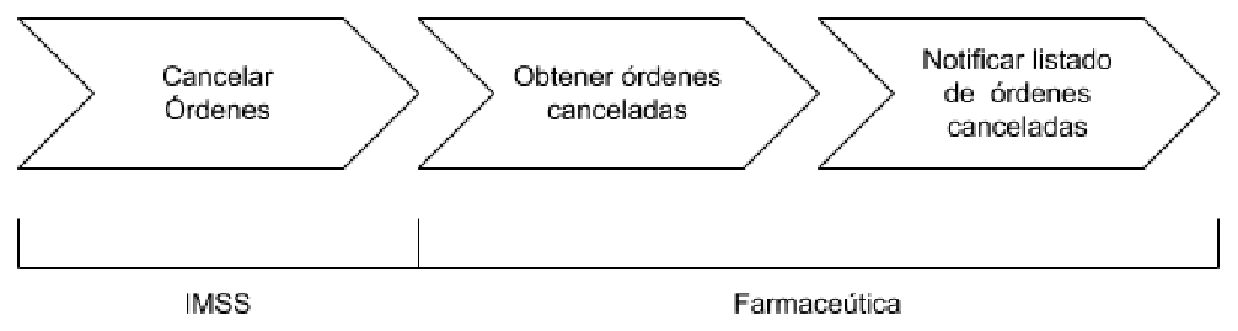
\includegraphics[scale=0.3]{flujo-proceso-verificar} 
\caption{Flujo del proceso para verificar órdenes de reposición canceladas.}
\label{fig:flow-proc-verificar}
\end{figure}
\end{itemize}

El proveedor que requiere automatizar la interacción con el portal SAI para el envío de las órdenes de reposición y la verificación de órdenes canceladas es una compañía farmacéutica por lo que en este documento nos referiremos al proveedor como la compañía farmacéutica, o simplemente farmacéutica. Los requerimientos funcionales del proveedor son la automatización de las tareas de interacción del operador con el portal SAI y la elaboración de reportes estadísticos sobre las órdenes de reposición procesadas durante la automatización.

\section{Justificación}
La farmacéutica atiende las órdenes de reposición del IMSS en el doble de tiempo que su competencia, en particular contestar estas órdenes en el portal SAI les toma hasta un día a tres personas dedicadas a ello.\\
La solución propuesta para acelerar la respuesta y verificación de órdenes de reposición en el portal SAI consiste en un sistema de software compuesto por agentes, donde cada agente se dedica a emular las acciones del operador de la farmacéutica, el cual es encargado de contestar o verificar las órdenes de reposición; cuenta con una base de datos donde se almacenen los datos capturados por lo agentes durante la respuesta de órdenes, y una interfaz gráfica donde los trabajadores de la farmacéutica puedan realizar tareas de administración: búsqueda, edición de órdenes de reposición y  generación de reportes de las órdenes atendidas por los agentes.\\
El proyecto de software anteriormente propuesto busca acortar el tiempo necesario para contestar las órdenes de reposición ayudando a mejorar el tiempo que toma a la farmacéutica atender las órdenes de reposición del IMSS, esto implica una reducción en tiempo desde que la orden es publicada en el portal SAI hasta que el medicamento es entregado físicamente al IMSS.\\
El segundo punto que soluciona este sistema es que evita el envío de medicamentos que ya no son solicitados, esto con el fin de evitar el consumo de recursos y el tiempo que toma retirar del IMSS tales medicamentos cancelados.\\
Los objetivos secundarios que conlleva este proyecto son:
\begin{enumerate}
\item Reducción del error humano en la manipulación de la información. 
\item Ahorro de recursos en entregas de medicamento no solicitado. 
\item Reducción de tiempo en la respuesta de órdenes de reposición.
\item Consistencia en los datos en la generación de reportes estadísticos sobre las órdenes de reposición procesadas.
\end{enumerate}
Por lo anterior los derechohabientes\footnote{Sec. Soc. Persona que se beneficia de ciertas prestaciones sociales por su vinculación con un seguro social: vínculo de parentesco (descendiente, ascendiente, consanguíneo), o de comunidad de vida, o de dependencia económica (persona a cargo. V. esta expresión).  http://www.enciclopedia-juridica.biz14.com/d/derechohabiente/derechohabiente.htm} del IMSS se verán beneficiados de los cambios hechos al nuevo sistema, pues los medicamentos estarán disponibles con mayor frecuencia en las clínicas y hospitales.

\section{Descripción general de trabajo}
La farmacéutica dedica diariamente un equipo de trabajo de 2 a 4 personas durante toda la jornada laboral, dependiendo del volumen de órdenes de reposición emitidas por el IMSS, para completar las tareas de envío de órdenes de reposición y verificar las órdenes de reposición canceladas dentro del portal SAI. A través del proyecto de automatización se pretenden optimizar los siguientes puntos:
\begin{itemize}
\item Reducción del esfuerzo de recursos humanos.
\item Eliminar errores de captura.
\item Reducción del tiempo dedicado a enviar las órdenes de reposición.
\item Detectar con rapidez las órdenes de reposición que hayan sido canceladas.
\end{itemize}
La necesidad de automatización de los procesos (ver Figuras \ref{fig:flow-proc-contestar} y \ref{fig:flow-proc-verificar}) antes mencionados pronostican una reducción de costos por devolución de medicamento no solicitado para el cliente y también la disminución de pérdidas en las ventas por solicitudes no atendidas en los rangos de tiempo acordados con el comprador. Dado lo anterior, se plantea un proyecto de software que cubra las necesidades de automatización y pueda ser administrado por usuarios no especializados en computación.\\
Para resolver el desarrollo del proyecto, el sistema se se divide en módulos con funcionalidades específicas que se muestran a continuación:
\begin{enumerate}
\item \textbf{Automatización de interacción con el portal SAI}. La automatización de la interacción con el portal SAI consiste emular los pasos que sigue una persona de la farmacéutica (operador) encargada de llenar y extraer información de las órdenes de reposición del portal SAI, es decir, listar los pasos que sigue el operador cuando contesta las órdenes de reposición, posteriormente describir las reglas de negocio necesarios para llenar los formularios que presenta el portal SAI al contestar una orden de reposición; por último, identificar las fuentes de los datos que se ocupan para llenar tales formularios y definir la forma de almacenar la información necesaria de cada formulario.
\item \textbf{Generación de reportes}. La generación de reportes consiste en plasmar la información obtenida de las órdenes de reposición contestadas en el módulo anterior, la farmacéutica tiene ya una plantilla que se utiliza para pasar los pedidos a otras áreas con el fin de continuar la atención de las órdenes de reposición, además de tal plantilla, la farmacéutica ha expresado el deseo de obtener estadísticas de la cantidad de órdenes de reposición atendidas y canceladas.
\item \textbf{Interfaz de usuario}. La interfaz de usuario se refiere a la aplicación que muestra una interfaz gráfica en la cual los operadores de la farmacéutica pueden solicitar la generación de reportes; hacer consultas y modificaciones a las órdenes de reposición atendidas por el primer módulo.
\end{enumerate}


\subsection{Arquitectura de la Solución}
La definición estricta de arquitectura de software es:
\begin{center}\textit{``El conjunto de estructuras necesarias para la comprensión de un sistema en el cual se comprometen elementos de software, relaciones entre ellos y sus propiedades''}\end{center}\footnote{Bourque, P. et. al. (2014). SWEBOK Guide V3.0. 1st. IEEE Computer Society.}
Tal definición lleva a pensar la arquitectura como el punto donde los requerimientos del cliente se traducen a especificaciones técnicas para los desarrolladores. En el caso del proyecto que se está presentando en este documento, la arquitectura está integrada por los siguientes componentes (ver Figura \ref{fig:dia-arq-comp}):
\begin{figure}[h]
\centering
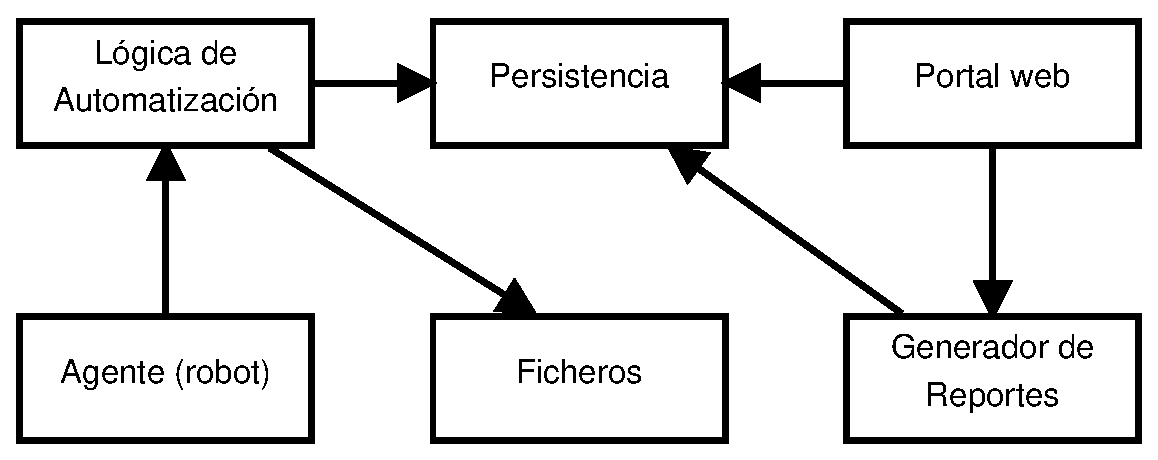
\includegraphics[scale=0.45]{dia-arq-comp} 
\caption{Módulos de la arquitectura.}
\label{fig:dia-arq-comp}
\end{figure}

\begin{itemize}
\item \textbf{Agente (robot)}. Interactúa directamente con el portal SAI, es el componente que automatiza las acciones de los operadores humanos de la farmacéutica.
\item \textbf{Lógica de negocio}. Son bibliotecas y rutinas que se encargan de prestar los servicios necesarios al agente para su funcionamiento, permite comunicación con la base de datos, guarda las capturas de pantalla en el sistema de archivos y provee la configuración de inicio al agente.
\item \textbf{Base de datos}. Es el componente que se encarga de llevar la persistencia de los datos obtenidos durante la respuesta a las órdenes de reposición.
\item \textbf{Sistema de archivos}. En el sistema de archivos se almacenan las capturas de pantalla al momento de enviar la respuesta de cada orden de reposición.
\item \textbf{Generador de reportes}. Este módulo está encargado de la generación de reportes tales como: órdenes de reposición atendidas, canceladas y formatos de órdenes de reposición enviadas.
\item \textbf{Portal web}. Portal mediante el cual los usuarios pueden hacer correcciones a los datos obtenidos de las órdenes de reposición, reimprimir el formato de envío de la orden de reposición  y descargar los reportes generados por el módulo generador de reportes.
\end{itemize}

\subsection{Plan de trabajo}
El proyecto será abordado con metodología Scrum, éste es un marco de trabajo para desarrollar, entregar y mantener productos complejos. Scrum consiste en un conjunto de roles, eventos, artefactos y reglas que los ligan. Scrum da un enfoque adaptivo mientras promueve la entrega continua de soluciones, y divide el desarrollo en ventanas de tiempo llamadas sprint\footnote{Schwaber, K. and Sutherland, J. (2017). The Scrum Guide. [online] Scrumguides.org. Disponible en: https://www.scrumguides.org/docs/scrumguide/v2017/2017-Scrum-Guide-US.pdf}.\\
La liberación del sistema consiste en el despliegue del total de los módulos en el ambiente productivo provisto por la farmacéutica,  dando como resultado los siguientes productos:
\begin{itemize}
\item Rutinas para la generación de objetos en base de datos.
\item Rutinas para la creación de la estructura de directorios en el sistema de archivos.
\item Archivos de configuración propio de cada módulo.
\item Herramienta de automatización y del automatización.
\item Bibliotecas del portal web.
\item Manual de instalación y de usuario.
\item Capacitación a usuarios finales.
\end{itemize}

\section{Índice}
\begin{enumerate}
  \item Introducción.
  \begin{enumerate}
    \item Contexto.
    \item Objetivo.
    \item Procedimiento manual de los operadores para contestar las órdenes de reposición.
  \end{enumerate}
  \item Análisis y alcance del proyecto.
  \begin{enumerate}
    \item Análisis de requerimientos.
    \begin{enumerate}
      \item Requerimientos funcionales.
      \item Requerimientos no funcionales.
    \end{enumerate}
    \item Alcance.
  \end{enumerate}
\item Diseño del proyecto.
\begin{enumerate}
  \item Diseño de la arquitectura.
  \item Diseño de la base de datos.
  \item Diseño de bibliotecas.
  \begin{enumerate}
    \item Diseño de rutinas de automatización.
  \end{enumerate}
  \item Diseño de servicios.
  \item Diseño de interfaz de usuario.
\end{enumerate}
\item Implementación.
\begin{enumerate}
  \item Implementación de base de datos.
  \item Implementación de bibliotecas.
  \begin{enumerate}
    \item Implementación de rutinas de automatización.
  \end{enumerate}
  \item Implementación de servicios.
  \item Implementación de interfaz de usuario.
\end{enumerate}
\item Liberación y resultados.
\item Conclusiónes.
\item Bibliografía.
\end{enumerate}

\section{Bibliografía propuesta}
\begin{enumerate}
\item Freeman, A. (2014). Pro AngularJS. 1st ed. Apress.
\item Josuttis, N. (2007), SOA in Practice, 1st ed. O’Reilly.
\item Evans, B. et. al. (2013). The Well-Grounded Java Developer. 1st ed. Manning.
\item Sarcar, V. (2016). Java Design Patterns, 1st ed. Apress.
\item Sierra, K. et. al. (2015). OCA/OCP Java SE 7, 1st ed. Oracle Press.
\item Gupta, M. (2013). OCA Java SE 7. 1st ed. Manning.
\item Gupta, M. (2015). OCP Java SE 7. 1st ed. Manning.
\item Scarioni, C. (2013). Pro Spring Security, 1st ed. Apress.
\item Walls, C. (2016). Spring Boot in Action. 1st ed. Manning.
\item Walls, C. (2015). Spring in Action. 4th ed. Manning.
\item Reddy, K. (2013). Java Persistence with MyBatis 3. 1st. Packt Publishing.
\item Siriwardena, P. (2014). Mastering Apache Maven 3. 1st. Packt Publishing.
\item Date, C. (2015). SQL and Relational Theory. 3rd. O’Reilly.
\item Bourque, P. et. al. (2014). SWEBOK Guide V3.0. 1st. IEEE Computer Society.
\item Schwaber, K. and Sutherland, J. (2017). The Scrum Guide. [online] Scrumguides.org. Disponible en: https://www.scrumguides.org/docs/scrumguide/v2017/2017-Scrum-Guide-US.pdf [Consultado 11  de agosto de 2018].
\item Kruchten, P. (1995). Architectural Blueprints—The “4+1” View Model of Software Architecture.  Disponible en: http://www.cs.ubc.ca/~gregor/teaching/papers/4+1view-architecture.pdf [Consultado 11 de agosto de 2018].
\item http://www.enciclopedia-juridica.biz14.com/d/derechohabiente/derechohabiente.htm
\end{enumerate}
 
\end{document}